\documentclass{article}
\usepackage{graphicx}
\usepackage[utf8]{inputenc}

\setlength\fboxsep{0pt}
\setlength\fboxrule{0.5pt}

\title{
    Requirements and Analysis Document for group 16
    \author{Erik Sjöström,
            Filip Labe,
            Jonatan Källman,
            Sarosh J. Nasir}
    \date{\today \\v1.0}         
}

\begin{document}
\maketitle

\section{Introduction}
Our project is a game about defeating monsters. You do this by clicking 
on the monsters with your finger. When defeated the monsters drop gold 
which can be used to buy upgrades. There are three upgrades that can be 
bought, upgrades to your damage, upgrades which provide damage every second 
or upgrades which provide gold every second. When the player has defeated enough 
monsters the player can progress to a new area and defeat monsters in a different 
scenery. 

\subsection{Definitions, acronyms, abbriviations}

\section{Requirements}
\subsection{User interface}
\subsection{Functional requirements}
\begin{itemize}
    \item Attack
    \item Open map
    \item Use map
    \item Buy upgrades
    \item Go home
    \item Improve home
    \item Check stats
\end{itemize}
\subsection{Non-functional requirements}
\subsubsection{Usability}
This will be a mobile game so we should put extra emphasis on the game being as
intuitive as possible.
\subsubsection{Performance}
The game should be light on resources.
\subsubsection{Implementation}
The application will be written in Java.
\subsection{Packaging and installation}
The application will be distributed as an \it{.apk}-file. 
\section{Use cases}
\subsection{Usability model}
\fbox{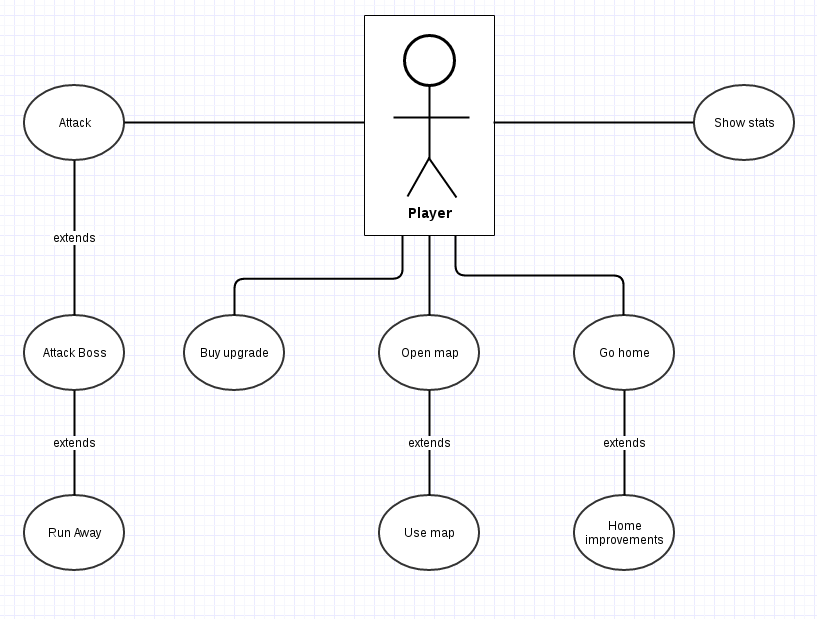
\includegraphics[scale=0.4]{usabilityModel.png}}
\subsection{Use case listings}
\subsubsection{Use case: Open app}
Summary: The user opens the app\\
Priority: High\\
Extends:\\
Includes:\\
Participators: User\\
\textbf{Normal flow of event:} The user opens the app and the game displays the main menu.
\vspace{1 mm}\\
\begin{tabular}{|c|l|l|} \hline
  & Actor & System \\ \hline
1 & User clicks app icon & \\ \hline
2 & & Load game \\ \hline
3 & & Display main menu \\ \hline
\end{tabular}\\
\vspace{5 mm}
\subsubsection{Use case: Attack}
Summary: The user clicks the screen and the game calculates new health for the monster.\\
Priority: High\\
Extends: undefined\\
Includes: undefined\\
Participators: Player\\
\textbf{Normal flow of event:} The player attacks the monster and the monster survives.
\vspace{1 mm}\\
\begin{tabular}{|c|l|l|} \hline
  & Actor & System \\ \hline
1 & Player clicks screen & \\ \hline
2 & & Calculate new health for monster\\ \hline
\end{tabular}\\
\newpage
\noindent
\textbf{Alternate flow:} The player attacks the monster and the monster dies. The level is not cleared.
\vspace{1 mm}\\
\begin{tabular}{|c|l|l|} \hline
    & Actor & System \\ \hline
    1 & Player clicks screen & \\ \hline
    2 & & Calculate new health for monster\\ \hline
    3 & & Replace dead monster with new monster \\ \hline
    4 & & Player gets money \\ \hline
\end{tabular}
\vspace{5 mm}\\
\textbf{Alternate flow:} The player attacks the monster and the monster dies. The level is cleared.
\vspace{1 mm}\\
\begin{tabular}{| c | l | l |} \hline
    & Actor & System \\ \hline
    1 & Player clicks screen & \\ \hline
    2 & & Calculate new health for monster\\ \hline
    3 & & Replace dead monster with new monster \\ \hline
    4 & & The option to change level is made avliable\\ \hline
    5 & & The player gets money \\ \hline
\end{tabular}
\\
\subsubsection{Use case: Attack boss}
Summary: The player is fighting a boss \\
Priority: High \\
Extends: Attack\\
Includes: \\
Participators: Player \\
\textbf{Normal flow of event:} The player attacks the boss and defeats it within the time frame 
\vspace{1 mm}\\
\begin{tabular}{|c|l|l|} \hline
    & Actor & System \\ \hline
    1 & Player clicks screen & \\ \hline
    2 & & Calculate new health for boss \\ \hline
    3 & & Unlock next level \\ \hline
    4 & & Player gets money \\ \hline
\end{tabular}
\newpage
\noindent
\textbf{Normal flow of event:} The player attacks the boss and does not defeat it, but is still within the time frame. 
\vspace{1 mm}\\
\begin{tabular}{|c|l|l|} \hline
    & Actor & System \\ \hline
    1 & Player clicks screen & \\ \hline
    2 & & Calculate new health for boss \\ \hline
\end{tabular}
\vspace{5 mm}\\
\textbf{Alternate event:} The player does not defeat the boss within the time frame 
\vspace{1 mm}\\
\begin{tabular}{|c|l|l|} \hline
    & Actor & System \\ \hline
    1 & & Reset boss \\ \hline
\end{tabular}

\vspace{5 mm}\\ 
\subsubsection{Use case: Open map}
Summary: The player clicks the map button
Priority: Medium \\
Extends: undefined\\
Includes: undefined\\
Participators: Player \\
\textbf{Normal flow of event:} The player clicks the map button\\
\begin{tabular}{|c|l|l|} \hline
      & Actor & System \\ \hline
    1 & Player clicks on the button & \\ \hline
    2 & & Displays map page \\ \hline
\end{tabular} 

\subsubsection{Use case: Use map}
Summary: The user tries to move to a different level.\\
Priority: High\\
Extends: undefined\\
Includes: undefined\\
Participators: Player \\
\textbf{Normal flow of event:} The player clicks on the level they want to move to, the level is unlocked.\\
\begin{tabular}{|c|l|l|} \hline
      & Actor & System \\ \hline
    1 & Player clicks on the level & \\ \hline
    2 & & Checks that the level is unlocked \\ \hline
    3 & & Loads new level \\ \hline
\end{tabular} \\
\textbf{Alternate flow of event:} The player clicks on the level they want to move to, the level is locked.
\vspace{1 mm}\\
\begin{tabular}{|c|l|l|} \hline
      & Actor & System \\ \hline
    1 & Player clicks on the level & \\ \hline
    2 & & Checks that the level is unlocked \\ \hline
\end{tabular} 

\subsubsection{Use case: Show stats}
Summary: The use clicks the stats button\\
Priority: low\\
Extends: undefined\\
Includes: undefined\\
Participators: Player\\
\textbf{Normal flow of event:} The player clicks the stats button
\vspace{1 mm}\\
\begin{tabular}{|c|l|l|} \hline
      & Actor & System \\ \hline
    1 & Player clicks on the button & \\ \hline
    2 & & Displays stats page \\ \hline
\end{tabular} 
\vspace{5 mm}
\subsubsection{Use case: Go home}
Summary: The user wants to go home\\
Priority: Low \\
Extends: undefined\\
Includes: undefined\\
Participators: Player \\
\textbf{Normal flow of event:} The player clicks the home button
\vspace{1 mm}\\
\begin{tabular}{|c|l|l|} \hline
      & Actor & System \\ \hline
    1 & Player clicks on the button & \\ \hline
    2 & & Displays the player home screen \\ \hline
\end{tabular} 
\vspace{5 mm}
\subsubsection{Use case: Home improvements}
Summary: The user wants to improve their home\\
Priority: low \\
Extends: undefined\\
Includes: undefined\\
Participators: Player\\
\textbf{Normal flow of event:} The player wants to buy an upgrade, has enough money.
\vspace{1 mm}\\
\begin{tabular}{|c|l|l|} \hline
      & Actor & System \\ \hline
    1 & Player clicks on a buy upgrade button & \\ \hline
    2 & & Deduct money from player \\ \hline
    3 & & Apply upgrade to player \\ \hline
\end{tabular}  
\vspace{5 mm}
\subsubsection{Use case: Buy upgrade}
Summary: The user is at the shop and wants to buy an upgrade.\\
Priority: Medium\\
Extends: undefined\\
Includes: undefined\\
Participators: Player\\
\textbf{Normal flow of event:} The player clicks on the upgrade and has enough money.
\vspace{1 mm}\\
\begin{tabular}{|c|l|l|} \hline
      & Actor & System \\ \hline
    1 & Player clicks on the upgrade & \\ \hline
    2 & & The upgrade is applied to the player \\ \hline
\end{tabular}

\section{Domain model}
\fbox{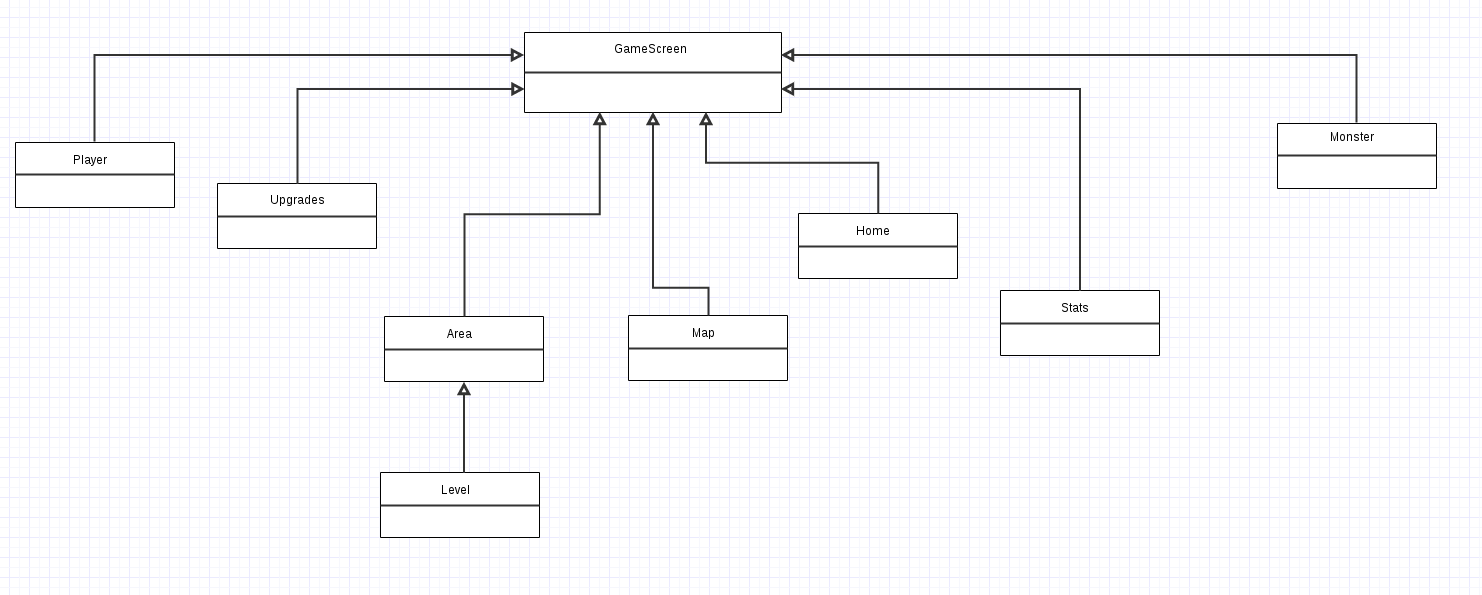
\includegraphics[scale=0.3]{domainModel.png}}

\subsection{Class responsibilities}
\subsubsection{Game screen}
Combines all other classes into one unified interface.
\subsubsection{Player}
The actual player. Has money, an amount of damage, an amount of damage per second and an amount of money per second.
\subsubsection{Monster}
A bad guy. Has health points, and an amount of money to drop.
\subsubsection{Stats}
A view for the players stats.
\subsubsection{Map}
A view for a map over the areas that a player can travel to.
\subsubsection{Upgrades}
A view over the upgrades that a player can buy.
\subsubsection{Home}
The players home. Here the player can upgrades which earn passive money. 
\subsubsection{Area}
An area, has a type, and a list of levels associated with that area.
\subsubsection{Level}
Determines how hard the monsters are, and how much money they drop.
\section{References}
No references yet.
\end{document}
